\documentclass[11pt, letterpaper]{article}
\setlength{\parindent}{0in}
\setlength{\textheight}{8.7in}
\setlength{\textwidth}{6.8in}
\setlength{\oddsidemargin}{-0.3in}
\setlength{\evensidemargin}{0.0in}
\addtolength{\topmargin}{-1in}
\setlength{\parskip}{0.1in}

\usepackage{amsmath, amsfonts, amssymb, color}
\usepackage{bm}
\usepackage{booktabs}
\usepackage{enumerate}
\usepackage{graphicx}
\usepackage{pdfpages}
\newcommand*{\justifyheading}{\raggedleft}


\renewcommand{\baselinestretch}{1.0}

\newcommand{\bx}{{\bm x}}
\newcommand{\bX}{{\bm X}}
\newcommand{\by}{{\bm y}}
\newcommand{\bY}{{\bm Y}}
\newcommand{\bW}{{\bm W}}
\newcommand{\bG}{{\bm G}}
\newcommand{\bR}{{\bm R}}
\newcommand{\bZ}{{\bm Z}}
\newcommand{\bV}{{\bm V}}
\newcommand{\bL}{{\bm L}}
\newcommand{\bz}{{\bm z}}
\newcommand{\be}{{\bm e}}
\newcommand{\bgamma}{{\bm \gamma}}
\newcommand{\bbeta}{{\bm \beta}}
\newcommand{\balpha}{{\bm \alpha}}
\newcommand{\bSigma}{{\bm \Sigma}}
\newcommand{\bmu}{{\bm \mu}}
\newcommand{\btheta}{{\bm \theta}}
\newcommand{\bepsilon}{{\bm \epsilon}}
\newcommand{\bone}{{\bm 1}}
\newcommand{\bzero}{{\bm 0}}
\newcommand{\bC}{{\bm C}}
\newcommand{\bI}{{\bm I}}
\newcommand{\bA}{{\bm A}}
\newcommand{\bB}{{\bm B}}
\newcommand{\bQ}{{\bm Q}}
\newcommand{\bS}{{\bm S}}
\newcommand{\bD}{{\bm D}}
\newcommand{\cQ}{\mathcal{Q}}
\newcommand{\cU}{\mathcal{U}}
\newcommand{\cI}{\mathcal{I}}
\newcommand{\cL}{\mathcal{L}}

\newcommand{\beas}{\begin{eqnarray*}}
\newcommand{\eeas}{\end{eqnarray*}}

\newenvironment{equationarrayright}{
                          \begin{eqnarray*}
                          \begin{array}{rcll}
                         }{
                          \end{array}
                          \end{eqnarray*}
                         }
\newcommand{\bear}{\begin{equationarrayright}}
\newcommand{\eear}{\end{equationarrayright}}

\renewcommand\arraystretch{1.3}

\DeclareMathOperator*{\argmin}{arg\,min}

\title{STAT/BIOST 571: Homework 3}
\author{Philip Pham}
\date{\today}

\begin{document}

\maketitle

\section*{Problem 1: Quasilikelihood and semiparametric methods for the general linear model (14 points)}
{\em This question examines the effect of different correlation structures, designs, and sample sizes in fitting a general linear model in a quasi-likelihood and semiparametric framework.  It is also an exercise in writing code systematically; please take care to break the required programming into small tasks, and write individual functions to do each of these tasks.
Please write all code ``by hand'', using matrix algebra and simple moment-based estimators.  
You may find the \texttt{mvtnorm} package helpful.

For the marginal model
\[
E(Y_{ij}|x_{ij}) = \beta_0 + \beta_1 x_{ij},
\]
consider estimation by weighted least squares, where the cluster weights are the inverse of
the estimated cluster covariance matrix.  Calculate quasi-likelihood standard errors as if your assumed form
of the covariance matrix
is known to be correct (even if, in actuality, you have assumed the wrong form of the covariance) and semi-parametric  standard errors using the sandwich estimator that accounts for clustering.
All of the notation follows the lecture notes. 

Throughout, the following are true in the data-generating mechanism
\begin{itemize}
\item $\beta_0=0$, $\beta_1 = 0.5$
\item $\bY_i|\bX_i\sim N(\bX_i \bbeta, \sigma^2 \bR_i)$ with $\sigma^2=1$. 
\end{itemize}
The factors that will vary are
\begin{itemize}
\item The number of clusters is 15, 30, or 60
\item The design: \begin{itemize}
\item Design I has $m_i = 4$, for all clusters. In each cluster, we see $\{x_{i1}, x_{i2},x_{i3},x_{i4}\}=\{7,10,13,16\}$
\item Design II has $m_i=3$ for all clusters.  We see equal numbers of clusters with $\{x_{i1}, x_{i2},x_{i3}\}=\{7,10,13\}, \{7,10,16\}, \{7, 13, 16\}, \textrm{ or }\{10, 13, 16\}$
\end{itemize}
\item The true covariance and the assumed covariance matrices are of the form $\sigma^2 \bR_i$:
\begin{itemize}
\item For the true covariance, consider exchangeable and exponential correlation structures, with $\rho=0.5$ or $\rho=0.9$ (distances between observations in the exponential model based on $x_{ij}$). 
\item For the assumed covariance, consider these and additionally the uncorrelated homoscedastic covariance.  Any covariance parameters should be estimated  using moment-based methods.
\end{itemize}
\end{itemize}}

\begin{table}
  \tiny
\centering
\begin{tabular}{ccr|ccc|ccc|ccc}
&&&\multicolumn{3}{|c}{$\mathbf{SD(\hat\beta_1)}$}&\multicolumn{3}{|c}{$\mathbf{E(\widehat{SE}_{1,QL})}$}&\multicolumn{3}{|c}{$\mathbf{E(\widehat{SE}_{1,sand})}$}\\
&&&\multicolumn{3}{c}{Assumed Corr}&\multicolumn{3}{|c}{Assumed Corr}&\multicolumn{3}{|c}{Assumed Corr}\\
$n$ & Design & True Corr & Uncor & Exch & Expon & Uncor & Exch & Expon & Uncor & Exch & Expon \\ \hline
15 &  I & Exchangeable $\rho=0.5$ & 0.03849 & 0.02853 & 0.03791 & 0.03768 & 0.02768 & 0.03702 & 0.02571 & 0.02571 & 0.02616 \\
15 &  I & Exchangeable $\rho=0.9$ & 0.03849 & 0.01466 & 0.02461 & 0.03698 & 0.01376 & 0.02319 & 0.0115 & 0.0115 & 0.01205 \\
15 &  I &         Exponential $\rho=0.5$ & 0.03849 & 0.03174 & 0.03799 & 0.03766 & 0.03088 & 0.0371 & 0.03619 & 0.03619 & 0.03577 \\
15 &  I &         Exponential $\rho=0.9$ & 0.03849 & 0.0174 & 0.02468 & 0.03707 & 0.01639 & 0.02334 & 0.02026 & 0.02026 & 0.02001 \\ [1ex]
15 & II & Exchangeable $\rho=0.5$ & 0.04464 & 0.03459 & 0.04015 & 0.04401 & 0.03372 & 0.03934 & 0.03493 & 0.03174 & 0.03213 \\
15 & II & Exchangeable $\rho=0.9$ & 0.04465 & 0.01899 & 0.025 & 0.04305 & 0.01797 & 0.02369 & 0.02588 & 0.0143 & 0.01475 \\
15 & II &         Exponential $\rho=0.5$ & 0.04472 & 0.03654 & 0.04025 & 0.04412 & 0.03581 & 0.03954 & 0.03911 & 0.03748 & 0.03737 \\
15 & II &         Exponential $\rho=0.9$ & 0.0447 & 0.0204 & 0.02468 & 0.04402 & 0.0197 & 0.02385 & 0.02892 & 0.01942 & 0.01922 \\ [2ex]
30 &  I & Exchangeable $\rho=0.5$ & 0.02722 & 0.01968 & 0.02682 & 0.0269 & 0.01936 & 0.02647 & 0.01857 & 0.01857 & 0.01897 \\
30 &  I & Exchangeable $\rho=0.9$ & 0.02722 & 0.00947 & 0.0161 & 0.02677 & 0.0092 & 0.01567 & 0.00839 & 0.00839 & 0.0088 \\
30 &  I &         Exponential $\rho=0.5$ & 0.02722 & 0.02213 & 0.02684 & 0.02705 & 0.02193 & 0.02664 & 0.02634 & 0.02634 & 0.02606 \\
30 &  I &         Exponential $\rho=0.9$ & 0.02722 & 0.01157 & 0.01624 & 0.02655 & 0.01116 & 0.01567 & 0.01459 & 0.01459 & 0.01444 \\ [1ex]
30 & II & Exchangeable $\rho=0.5$ & 0.03148 & 0.02376 & 0.02816 & 0.03134 & 0.0235 & 0.02793 & 0.02525 & 0.02283 & 0.02316 \\
30 & II & Exchangeable $\rho=0.9$ & 0.03152 & 0.01201 & 0.01598 & 0.03104 & 0.01172 & 0.0156 & 0.01902 & 0.01018 & 0.01051 \\
30 & II &         Exponential $\rho=0.5$ & 0.03148 & 0.02534 & 0.02813 & 0.03138 & 0.02514 & 0.02795 & 0.02906 & 0.02776 & 0.02766 \\
30 & II &         Exponential $\rho=0.9$ & 0.03158 & 0.01322 & 0.01588 & 0.03143 & 0.01302 & 0.01564 & 0.02119 & 0.01408 & 0.0139 \\ [2ex]
60 &  I & Exchangeable $\rho=0.5$ & 0.01925 & 0.0138 & 0.01895 & 0.01916 & 0.0137 & 0.01885 & 0.01339 & 0.01339 & 0.01367 \\
60 &  I & Exchangeable $\rho=0.9$ & 0.01925 & 0.00641 & 0.01103 & 0.01901 & 0.00629 & 0.01082 & 0.00599 & 0.00599 & 0.00629 \\
60 &  I &         Exponential $\rho=0.5$ & 0.01925 & 0.01554 & 0.01893 & 0.01913 & 0.01543 & 0.01881 & 0.0188 & 0.0188 & 0.0186 \\
60 &  I &        Exponential $\rho=0.9$ & 0.01925 & 0.00793 & 0.01099 & 0.01909 & 0.00782 & 0.01084 & 0.01057 & 0.01057 & 0.01045 \\ [1ex]
60 & II & Exchangeable $\rho=0.5$ & 0.02225 & 0.01661 & 0.01983 & 0.02212 & 0.01648 & 0.01969 & 0.01779 & 0.01615 & 0.01635 \\
60 & II & Exchangeable $\rho=0.9$ & 0.02224 & 0.008 & 0.01078 & 0.02201 & 0.00786 & 0.0106 & 0.01373 & 0.00734 & 0.00757 \\
60 & II &         Exponential $\rho=0.5$ & 0.02225 & 0.0178 & 0.01983 & 0.02213 & 0.01768 & 0.0197 & 0.02032 & 0.01953 & 0.01944 \\
60 & II &         Exponential $\rho=0.9$ & 0.02223 & 0.0089 & 0.01066 & 0.02208 & 0.00879 & 0.01053 & 0.01505 & 0.00997 & 0.00987
\end{tabular}
\caption{Table of standard deviations of the estimated slopes and 
  average of model-based and sandwich-based standard error estimates}
\label{tab:p1_results}
\end{table}

\begin{description}
\item[Solution:] See the results in Table \ref{tab:p1_results}. Correct standard
  errors are found when the assumed correlation structure agrees with the true
  correlation structure when using GLS (columns 2 and 3). Ignoring the
  correlation within the clusters overestimates the standard error (first
  column). When incorrectly assuming exponential correlation, the standard error
  is overestimated. When incorrectly assuming exchangeable correlation, the
  standard error is underestimated.

  Quasi-likelihood doesn't help very much when the correlation structure is
  misspecified. The standard error estimates are almost identical to just using
  GLS. The standard errors are slightly closer to those of the sandwich
  estimator, so there is some insignificant gain.

  Comparing the sandwich estimation with GLS when the assumed correlation is
  correct, one sees that the standard error estimates are underestimated for
  smaller $n$. For $n = 60$, the estimates are very good. When the correlation
  structure is misspecified, sandwich estimation comes closest to the actual the
  standard error, especially when $n$ is large (verified numerically, results
  not shown). It follows that misspecifying the correlation structure as
  exchangeable or exponential doesn't affect the standard error of
  $\hat{\beta}_1$ very much. 

  This is also the case when assuming no correlation with design I. However, when
  using design II, where not all the clusters have identical covariates,
  assuming no correlation increases the standard error of our estimator
  significantly. This effect is even more pronounced when there is more
  correlation ($\rho = 0.9$ versus $\rho = 0.5$).

  Details of the calculation are described below, and code is in the appendix.
    
  Let $X_i$ be the covariates for each cluster with a column of $1$s
  prepended. Let $y_i$ be the cluster responses.

  We first estimate $\beta$ with the ordinary least squares (OLS) estimator,
  $\hat{\beta}_{\mathrm{OLS}} = \left(X^\intercal X\right)^{-1}X^\intercal y$,
  where $X$ is the concatenation of the cluster covariates and $y$ is the
  concatenation of the cluster responses.
  
  We can get the covariances for $\hat{\beta}$ with
  \begin{align*}
    \operatorname{cov}\left(\hat{\beta}\right)
    &= \left(\sum_{i=1}^n X_i^\intercal W X_i\right)^{-1}
    \left(\sum_{i=1}^n X_i^\intercal W \hat{\Sigma} W X_i\right)
    \left(\sum_{i=1}^n X_i^\intercal W X_i\right)^{-1}.
  \end{align*}

  For the different estimation methods and assumed covariances, we vary the form
  of $\hat{\Sigma}$ and $W$, both of which are assumed to be the same for all
  clusters.

  To obtain $W$, we first estimate $\sigma^2$ with
  \begin{equation}
    \hat{\sigma}^2 = \frac{1}{\sum_{i=1}^nm_i - 2}\sum_{i=1}^n
    \left(y_{i} - X_{i}\hat{\beta}_{\mathrm{OLS}}\right)^\intercal
    \left(y_{i} - X_{i}\hat{\beta}_{\mathrm{OLS}}\right).
  \end{equation}


  Let the standardized OLS residuals for each cluster be
  $\tilde{\epsilon}_i = \frac{y_i -
    X_i\hat{\beta}_{\mathrm{OLS}}}{\hat{\sigma}}.$

  If we assume that the correlation structure is exchangeable, we estimate
  \begin{equation}
    \hat{\rho}_{\mathrm{exch}} =
    \frac{1}{\sum_{i=1}^n\sum_{j=1}^{m_i - 1} j}\sum_{i=1}^n\sum_{j=1}^{m_i - 1}\sum_{k=j + 1}^{m_i}
    \left(\tilde{\epsilon}_i\tilde{\epsilon}_i^\intercal\right)_{jk},
  \end{equation}
  so $W^{-1}_{ii} = 1$ for all $i$ and
  $W_{ij}^{-1} = \hat{\rho}_{\mathrm{exch}}$ for all $i \neq j$.

  If we assume that the correlation structure is exponential, we estimate
  \begin{equation} \hat{\rho}_{\mathrm{expon}} =
    \frac{1}{\sum_{i=1}^n\sum_{j=1}^{m_i - 1}
      j}\sum_{i=1}^n\sum_{j=1}^{m_i - 1}
    \left(\tilde{\epsilon}_i\tilde{\epsilon}_i^\intercal\right)_{j,j+1},
  \end{equation}
  so
  $W_{ij}^{-1} = \hat{\rho}_{\mathrm{expon}}^{\left\lvert j - i \right\rvert}$
  for any $i$ and $j$.
  
  If we don't assume any correlation structure, $W = I$.

  Now that we know $W$, we can estimate $\beta$ with
  \begin{equation}
    \hat{\beta} = \frac{1}{\sum_{i=1}^nm_i}\sum_{i=1}^nm_i\left(X_i^\intercal W X_i\right)^{-1} X_i^\intercal W y_i.
  \end{equation}
  
  By default, for the general linear model, we would have that
  $\hat{\Sigma} = W^{-1}$, in which case, we have that
  \begin{equation}
    \operatorname{cov}\left(\hat{\beta}\right)
    = \left(\sum_{i=1}^n X_i^\intercal W X_i\right)^{-1}.
  \end{equation}

  In the quasi-likelihood model, we have an additional dispersion factor
  $\alpha$, so $\hat{\Sigma} = \hat{\alpha}W^{-1}$, where
  \begin{equation}
    \hat{\alpha} = \frac{1}{\sum_{i=1}^n m_i - 2}
    \left(y - X\hat{\beta}\right)^\intercal\left(y - X\hat{\beta}\right),
  \end{equation}
  which results in the covariance
  \begin{equation}
    \operatorname{cov}\left(\hat{\beta}\right)
    = \hat{\alpha} \left(\sum_{i=1}^n X_i^\intercal W X_i\right)^{-1}.
  \end{equation}

  For the sandwich estimator, we use the empirical estimate
  \begin{equation}
    \hat{\Sigma} = \frac{1}{n}\sum_{i=1}^n
    \left(y_i - X_i\hat{\beta}\right)^\intercal \left(y_i - X_i\hat{\beta}\right).
  \end{equation}
  
\end{description}

\section*{Problem 2: Efficiency of OLS for linear models with correlated data (6 points)}
{\em Review the example on slides 2.34 -- 2.35, which can also be found on pages 60 -- 62 of the Diggle et al. textbook.  We will generalize this example by considering the mean model
\[
E(Y_{ij}) = \beta_0 + \beta_1 x_j
\]
for arbitrary $\bx = (x_1,x_2,\ldots,x_5)$ that is the same for all subjects, but which may or may not
be equal to ${\bm t}=(-2,-1,0,1,2)$ (as is the case in the original version of the example).
Note that the correlation structure is still determined based on $t$, as in the original example, but now the mean model contains $x$ rather than $t$.}
\begin{enumerate}[(a)]
{\em \item Derive a general expression for the relative efficiency of OLS compared to the optimal GLS in estimating $\beta_0$ and $\beta_1$ in this problem.  Your formula should be valid for a homoscedastic exponential covariance matrix with arbitrary
$\rho$ and for arbitrary $\bx$.  That is, derive a general version of the expressions
on the bottom of 2.44 that is valid for any choice of covariates.  Note that it is acceptable for your solution to be written using matrix notation and matrix algebra.}

\begin{description}
\item[Solution:] Let there be $n$ subjects. Each subject $i$ has $m_i$
  observations
  $x_i = \begin{pmatrix} x_{i1} & 
    x_{i2} & \ldots & x_{im_i} \end{pmatrix}^\intercal$. Let $X_i$ be the
  $m_i \times 2$ covariate matrix, where $X_{ij1} = 1$ and $X_{ij2} =
  x_{ij}$. Let $X$ be the $\sum_{i=1}^n m_i \times 2$ matrix obtained by
  stacking $X_1,X_2,\ldots, X_n$.

  The true model is $Y_{ij} = \beta_0 + \beta_1x_{ij} + \epsilon_{ij}$. Let the
  obvervations between subjects be independent with each other. Let $\Sigma_i$
  denote the covariance structure for within-subject observations, that is
  $\Sigma_{ijk} = \operatorname{cov}\left(\epsilon_{ij}, \epsilon_{ik}\right)$.
  Let $\Sigma$ be the $\sum_{i=1}^n m_i \times \sum_{i=1}^n m_i$ block diagonal
  matrix
  \begin{equation}
    \Sigma =
    \begin{pmatrix}
      \Sigma_1 & & & \\
      & \Sigma_2 & & \\
      & & \ddots & \\
      & & & \Sigma_n
    \end{pmatrix}.
  \end{equation}
  Let $Y_i$ be the vector of observations for subject $i$. Let $Y$ be obtained
  by concatenating the $Y_1,Y_2,\ldots,Y_n$. If
  $\beta = \begin{pmatrix} \beta_0 & \beta_1 \end{pmatrix}^\intercal$, we can
  write $Y = X\beta + \epsilon$, where
  $\epsilon \sim \mathcal{N}\left(\mathbf{0}, \Sigma\right)$.
    
  The OLS estimate for is
  \begin{equation}
    \hat{\beta}_{\mathrm{OLS}} = \left(X^{\intercal}X\right)^{-1}X^\intercal Y
    = \beta + \left(X^{\intercal}X\right)^{-1}X^\intercal \epsilon,
  \end{equation}
  which has covariance
  \begin{align}
    \operatorname{cov}\left(\hat{\beta}_{\mathrm{OLS}}\right)
    &= \left(X^{\intercal}X\right)^{-1}X^\intercal
    \operatorname{cov}\left(\epsilon\right)
      X\left(X^{\intercal}X\right)^{-1} \nonumber\\
    &= \left(X^{\intercal}X\right)^{-1}X^\intercal
      \Sigma
      X\left(X^{\intercal}X\right)^{-1}.
      \label{eqn:p2_beta_hat_ols}
  \end{align}

  The optimal GLS estimate, which can be derived by maximizing likelihood is
  \begin{equation}
    \hat{\beta}_{\mathrm{GLS}} = \left(X^{\intercal}\Sigma^{-1}X\right)^{-1}X^\intercal\Sigma^{-1} Y
    = \beta + \left(X^{\intercal}\Sigma^{-1}X\right)^{-1}X^\intercal\Sigma^{-1} \epsilon,
  \end{equation}
  which has covariance
  \begin{align}
    \operatorname{cov}\left(\hat{\beta}_{\mathrm{GLS}}\right)
    &= \left(X^{\intercal}\Sigma^{-1}X\right)^{-1}X^\intercal
      \Sigma^{-1}
      \operatorname{cov}
      \left(\epsilon\right)
      \Sigma^{-1}
      X\left(X^{\intercal}\Sigma^{-1}X\right)^{-1} \nonumber\\
    &= \left(X^{\intercal}\Sigma^{-1}X\right)^{-1}.
      \label{eqn:p2_beta_hat_gls}
  \end{align}

  Much of these matrix multiplications can be written as summations:
  \begin{align*}
    X^\intercal X
    &= \sum_{i=1}^n X_i^\intercal X_i \\
    X^\intercal \Sigma X
    &= \sum_{i=1}^n X_i^\intercal \Sigma_i X_i \\
    X^\intercal \Sigma^{-1} X
    &= \sum_{i=1}^n X_i^\intercal \Sigma_i^{-1} X_i.,
  \end{align*}
  which is probably computationally faster if $n$ is very large.

  In any case, using Equations \ref{eqn:p2_beta_hat_ols} and
  \ref{eqn:p2_beta_hat_gls}, we can calculate relative efficiency
  \begin{align*}
    e\left(\hat{\beta}_0\right)
    &= \left.
      \left[\left(X^{\intercal}\Sigma^{-1}X\right)^{-1}\right]_{11}
      \middle/
      \left[\left(X^{\intercal}X\right)^{-1}X^\intercal
      \Sigma
      X\left(X^{\intercal}X\right)^{-1}\right]_{11}
      \right. \\
    e\left(\hat{\beta}_1\right)
    &= \left.
      \left[\left(X^{\intercal}\Sigma^{-1}X\right)^{-1}\right]_{22}
      \middle/
      \left[\left(X^{\intercal}X\right)^{-1}X^\intercal
      \Sigma
      X\left(X^{\intercal}X\right)^{-1}\right]_{22}
      \right.
  \end{align*}
  by taking the corresponding entries of the covariance matrix.
\end{description}
{\em \item Reproduce the lines in the table on 2.35 that pertain to $\beta_1$ for the following choices of covariate vectors
\beas
\bx&=&(-2,-1,0,1,2)\\
\bx&=&(-1,-2,0,2,1)\\
\bx&=&(0,-1,1,3,2)\\
\bx&=&(0,-1,1,5,2)
\eeas}


\begin{table}[ht!]
  \scriptsize
  \centering
  \begin{tabular}{llllllllllll}
\toprule
                 & $\rho$ &    0.1 &    0.2 &    0.3 &    0.4 &    0.5 &    0.6 &    0.7 &    0.8 &    0.9 &   0.99 \\
$x$ & Value &        &        &        &        &        &        &        &        &        &        \\
\midrule
(-2, -1, 0, 1, 2) & $e(\hat{\beta}_0)$ & 0.9978 & 0.9917 &  0.983 & 0.9729 & 0.9631 & 0.9554 & 0.9521 & 0.9558 & 0.9701 & 0.9961 \\
                 & $e(\hat{\beta}_1)$ & 0.9969 & 0.9893 & 0.9797 &   0.97 & 0.9615 & 0.9554 & 0.9522 & 0.9522 & 0.9554 & 0.9608 \\
(-1, -2, 0, 2, 1) & $e(\hat{\beta}_0)$ & 0.9978 & 0.9917 &  0.983 & 0.9729 & 0.9631 & 0.9554 & 0.9521 & 0.9558 & 0.9701 & 0.9961 \\
                 & $e(\hat{\beta}_1)$ & 0.9959 & 0.9818 & 0.9554 & 0.9154 & 0.8621 & 0.7974 & 0.7249 & 0.6486 & 0.5726 &  0.507 \\
(0, -1, 1, 3, 2) & $e(\hat{\beta}_0)$ & 0.9972 & 0.9888 & 0.9758 & 0.9596 & 0.9432 & 0.9302 & 0.9247 &  0.931 & 0.9541 & 0.9942 \\
                 & $e(\hat{\beta}_1)$ & 0.9959 & 0.9818 & 0.9554 & 0.9154 & 0.8621 & 0.7974 & 0.7249 & 0.6486 & 0.5726 &  0.507 \\
(0, -1, 1, 5, 2) & $e(\hat{\beta}_0)$ & 0.9949 & 0.9817 & 0.9636 & 0.9445 & 0.9281 & 0.9178 & 0.9169 & 0.9279 & 0.9541 & 0.9943 \\
                 & $e(\hat{\beta}_1)$ & 0.9911 & 0.9644 & 0.9206 & 0.8626 &  0.794 & 0.7194 & 0.6432 & 0.5689 & 0.4992 & 0.4416 \\
\bottomrule
\end{tabular}

  \caption{Efficiency results comparing OLS with GLS.}
  \label{tab:p2_efficiencies}
\end{table}

\begin{description}
\item[Solution:] Results can be seen Table \ref{tab:p2_efficiencies}. Code is in the appendix.
\end{description}

{\em \item Explain the key differences between the relative efficiencies you just calculated.  Phrase your answers in a manner that will be understandable by
a quantitavely sophisticated non-statistician (e.g., an epidemiologist collaborator).
}

\begin{description}
\item[Solution:] If there's not much correlation, i.e. small $\rho$, there's not
  much efficiency gain in using GLS over OLS.

  For $\beta_1$, the efficiency gain does depend on the observed covariates,
  however. Recall that the estimated for $\beta_1$ can be written as a sum of
  weighted pairwise slopes. The weight is higher for for pairs where $x_{ij_1}$
  and $x_{ij_2}$ are further part because the effect size becomes bigger
  relative to the noise. Similarly, when the errors are positively correlated,
  more of the variance is explained away, so we are more confident about the
  slope estimate $\beta_1$.

  These two factors interact multiplicatively. Thus, when
  \[\mathbf{x} \in \left\{ (-1,-2,0,2,1), (0,-1,1,3,2), (0,-1,1,5,2) \right\},\]
  there are pairs of observations where the difference in covariates is large
  and the correlation is high. GLS is able to leverage this to produce a more
  efficient estimator. In particular when $\mathbf{x} = (0,-1,1,5,2)$, there are
  neighboring observations where the difference in covariates can be quite
  large, leading to the relatively most efficient estimator when using GLS.
\end{description}
\end{enumerate}

\section*{Appendix}

Code is attached on subsequent pages.

\clearpage

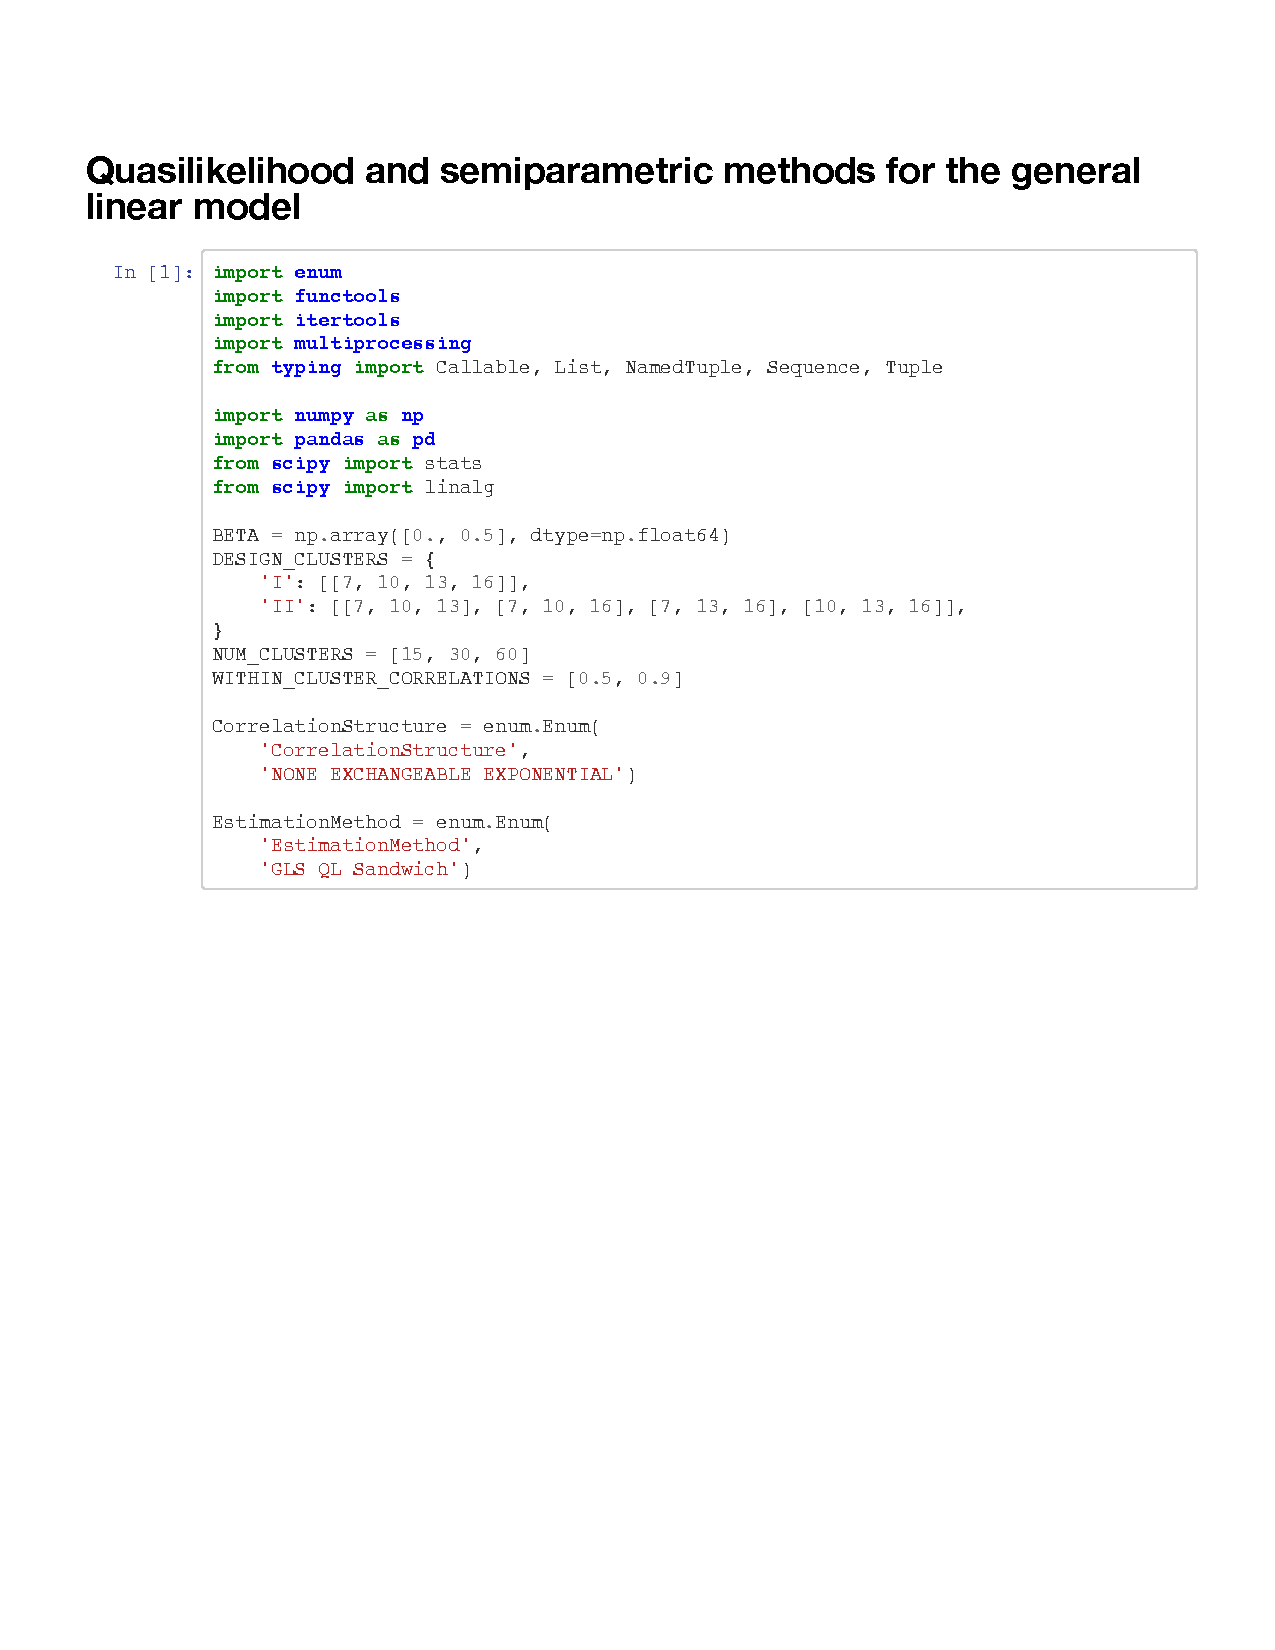
\includepdf[pages=-]{p1_glm.pdf}
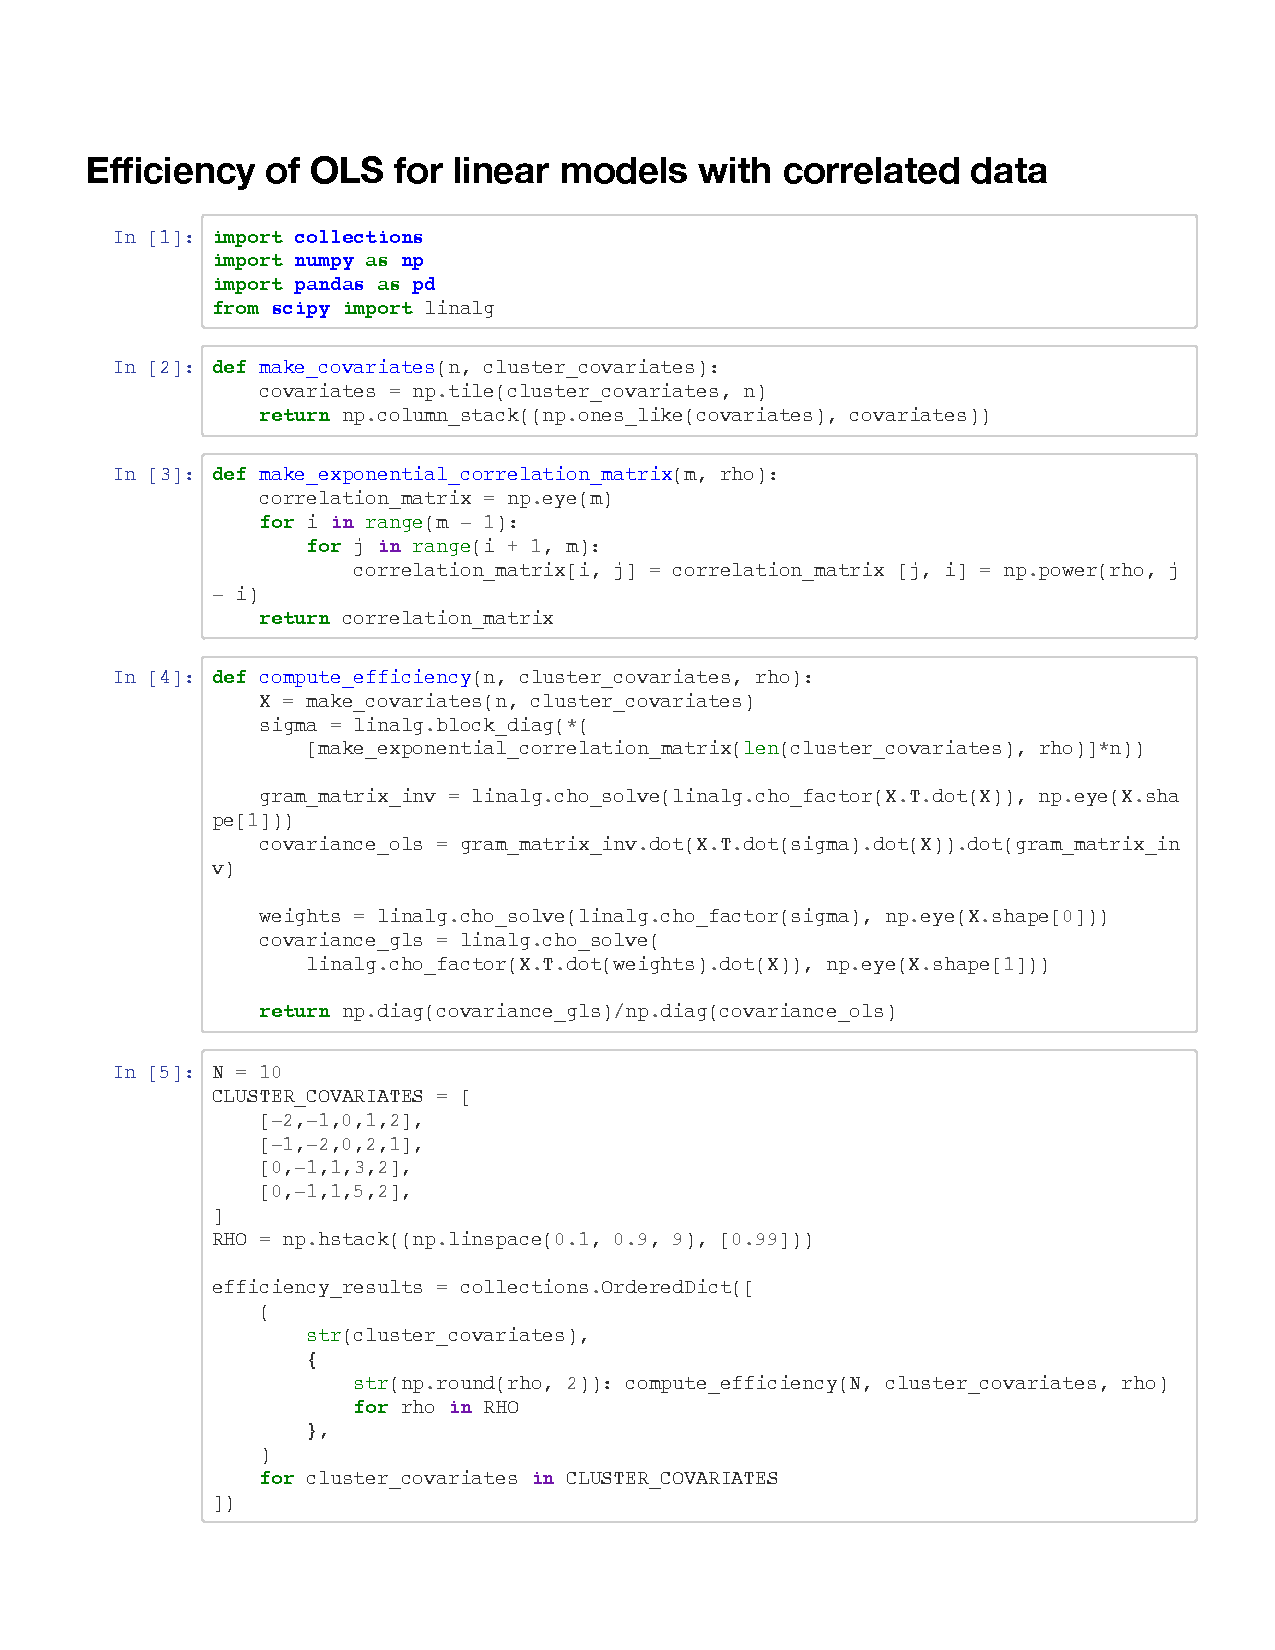
\includepdf[pages=-]{ols_efficiency.pdf}

\end{document}